\documentclass[conference]{IEEEtran}

% \usepackage[a-2u]{pdfx}% To generate PDF/A standard.
% \usepackage{cite}
\usepackage{hyperref}
\usepackage{graphicx}

\title{Real-Time Pothole Detection and Localization Using Convolutional Neural Network}

% \author{ATIKUR RAHMAN \\ chitholian@gmail.com}

\begin{document}
\maketitle
 
%To show page numbers with [conference] option in documentclass.
\thispagestyle{plain}
\pagestyle{plain}
%%%%%%%%%%%%%%%%%%% Abstract %%%%%%%%%%%%%%%%%%%
\begin{abstract}
  Pothole is a common problem in damaged roads and pavements. Vehicles get damaged, people get stumbled, drivers lose control over the car and accidents take place. A system is required that can detect potholes as fast as possible and help to avoid them. In this paper, such a system is being described which is capable of detecting potholes in video frames as well as localizing and tracking them. The system can also make instantaneous signal and warn about the detected potholes. It works in real-time even in mobile devices like android smart-phone. Convolutional Neural Network has been used as the basis of the model. A dataset was prepared where images having potholes were annotated by selecting the regions containing potholes. Following an approach of supervised transfer-learning, a neural network model was developed. The model was then deployed as android application for real-world testing purpose. Satisfactory result was found in both theoretical evaluation and practical real-world tests.
\end{abstract}
 
%%%%%%%%%%%%%%%%%%% Keywords %%%%%%%%%%%%%%%%%%%
\begin{IEEEkeywords}
  Pothole, Detection, Localization, Real-Time, ConvNet, CNN, Neural Net, Fine-Tuning, Transfer Learning.
\end{IEEEkeywords}

%%%%%%%%%%%%%%%%%%% Introduction %%%%%%%%%%%%%%%%%%%
\section{Introduction}
According to Cambridge Dictionary\cite{walter2008cambridge} a pothole is ``a hole in a road surface that results from gradual damage caused by traffic and/or weather''. Potholes cause huge trouble in regular transportation system. Vehicles may get damaged when they hit pothole. People who are visually impaired face a great problem due to potholes while navigating. Sometimes drivers may lose their control over the car and result in accidents. Therefore, to get rid of this problem either potholes must be repaired as soon as they appear or drivers and passers-by must be aware of them during navigation so that they can be avoided or passed safely.
  
Although the first one is very inefficient and troublesome, research have taken place to detect potholes and mark the location where they occurred\cite{yu06,zoysa07,li09,buza2013stereo,koch11}. The collected data then is sent to the authority so that the hole is repaired soon. Second one is also researched on\cite{rao16,danti12}, to inform navigators about the potholes appearing on the road surface in front of them.
  
This research is also focused on the second one, i.e. detect potholes before you hit them and try to avoid if possible or hit safely. The research work targets to develop a system for automatic detection of potholes in real-time and generate signal to warn about them.
  
A supervised learning approach\cite{kotsiantis2007supervised} was followed along with transfer learning\cite{pan2009survey} in this research to build the detector model. A dataset of annotated images was used to train and evaluate the model. Pre-trained MobileNet\cite{howard2017mobilenets}, a Convolutional Neural Network model was used as the feature extractor. Single Shot Multibox Detector (SSD)\cite{liu2016ssd} was fine-tuned for detection and localization of potholes. Despite training on image dataset, the resulting model is capable of detecting, localizing and tracking potholes in real-time analyzing the video frames.
  
An android application has been developed using the model which can detect, localize and track the potholes in the video coming from its camera. It also generates warning signal as long as pothole is detected in the video stream. Thus, it is very helpful for blind people to navigate. Localization capability of potholes in video stream can be very useful in case of automated vehicle driving.
  
In this paper, explanation and discussion of technical requirements, materials and methods, results and evaluation of our research is given following a review of existing and related works. After all, conclusion and future works are given followed by the bibliography.
  
%%%%%%%%%%%%%%%%%%% Related Works %%%%%%%%%%%%%%%%%%%
\section{Related Works}
Mednis et al. proposed such a mobile sensing system for road\cite{rao16} which was able to detect inconsistency with the help of a smartphone based on Android Operating System\cite{mednis11,rao16}. They took a 4.4 km long track for the testing purpose with 10 consecutive laps. Using real-world data, their method presented around 90\% True Positive Rate (TPR)\cite{kim14}.
    
This method could result in wrong information for the cases such as---
\begin{itemize}
  \item {It detects hinges as well as joints of the road\cite{kim14} as pothole event if it is not the case though.}
        \item{It fails to detect potholes which are in the middle of the lane.}
\end{itemize}
    
Chang et al. showed that scanning as well as extracted focusing on some particular distress features were captured along with accurate 3D cloud points with their elevation by means of a grid-based approach\cite{chang05}. Severity and coverage of the distress could be accurately and automatically calculated using this method\cite{chang05,kim14}.
    
Li et al. presented an inspection system\cite{li09} which can be used to detect and identify distress features like potholes, shoving and rutting with the help of a 3D transverse scanning technique\cite{li09} and it is a high-speed technology. The technique mentioned uses infrared waves featured laser line projector with a digital camera for detecting distress features as well as potholes\cite{li09}. 
            
Joubert et al.\cite{buza2013stereo} proposed a low-cost sensor system using Kinect sensor and high speed USB camera\cite{buza2013stereo} to detect and analyze potholes. Some experiments have already taken place on using Kinect to examine potholes. This method is cost-effective which is a plus-point.
            
Buza et al.\cite{buza2013stereo} proposed an unsupervised method using computer vision which does not require expensive equipment, filtering or training phases\cite{buza2013stereo,ryu2015image}. They used general image processing and clustering technologies for detecting and identifying potholes in the target image\cite{kim14}.
    
Their method consists of three steps as given below---
\begin{enumerate}
  \item {Segmentation of Target Images}
  \item {Shape and Feature Extraction}
  \item {Detection and Identification}
\end{enumerate}
Using the method stated above they reached an accuracy of 81\%\cite{kim14} and it could be used as a rough estimation for pothole-repairs.
    
Lokeshwor et al.\cite{huidrom2013method} proposed a method which could detect potholes, cracks and patches of pavement by analyzing video frames. Using DFS algorithm\cite{huidrom2013method,kim14}, they segmented video clips undoubtedly into two frames namely, stressed and distressed categories.
    
Jog et al.\cite{jog2012pothole} showed a system for 2D recognition and 3D reconstruction\cite{jog2012pothole} to detect and measure potholes along with their severity. They used video camera seated on the car to capture video of pavements.
    
They were able to find the depth, width and number of potholes using this approach.
    
Koch and Brilakis\cite{koch2013pothole} proposed a method which was bound to single frame of the video coming form camera. It could not find the magnitude of potholes analyzing the frames of pavement video-frames\cite{kim14}.
Koch et al. showed an updated composition signature for perfect pavement regions for pothole recognition. They also applied computer vision for tracking detected potholes in the all video frames\cite{koch2013pothole}.
 
%%%%%%%%%%%%%%%%%%% Technical Requirements %%%%%%%%%%%%%%%%%%%
\section{Technical Requirements}
The following technical requirements were identified for the research, preliminary system development, testing and deployment---
\begin{enumerate}
  \item A dataset of images is required to be fed the model for training purpose. In case of video, frames can be extracted\cite{schultz1996extraction} as images and must be annotated.
           
  \item Dataset images must be annotated in such a way that the regions of interest i.e. image-areas having pothole must be selected e.g. as bounding-boxes\cite{lempitsky2009image}.
           
  \item For model train-up, a digital workstation\cite{pirkle1988computer} computer is recommended with ``at least'' following configurations---
        \begin{itemize}
          \item CPU: 2.2 GHz (6\textsuperscript{th} Gen)
          \item RAM: 16 GB (2400 MHz DDR4)
          \item GPU:
                \begin{itemize}
                  \item VRAM: 12GB
                  \item Computing\cite{owens2008gpu} Capability: 5
                  \item CUDA\cite{kirk2007nvidia} support.
                \end{itemize}
        \end{itemize}
        However, model developed in this research was trained on the Google Colaboratory\cite{bisong2019google}.
           
  \item Android\cite{android2011android} Smartphone with speaker and camera support. Android OS version $\geq 6$ (Marshmallow, API 22).
\end{enumerate}

%%%%%%%%%%%%%%%%%%% Materials and Methods %%%%%%%%%%%%%%%%%%%
\section{Materials and Methods}
\subsection{The Dataset}
We have used a novel (custom) dataset of images. A portion (57.1\%) of the dataset images was scrapped from Google Image Search. The rest (42.9\%) was captured with an Android smartphone camera from some damaged roads in the campus of University of Chittagong. 
   
The dataset contains total 665 images having a total of 1740 annotated potholes. Each image was annotated with bounding boxes around the regions having potholes. For this purpose, labelImg\cite{tzutalingit} was used as the annotation tool.
   
The training set contains 532 (80\%) images and the test set contains 133 (20\%) images. The potholes were divided into three categories---
\begin{enumerate}
  \item Small
  \item Medium
  \item Large
\end{enumerate}
   
The sizes of the potholes were measured from the occupied pixels in the sample images. 
The number of pixels occupied was calculated after resizing the longer side of the images to 300px keeping the aspect ratio of the shorter side.
   
The number of pixels occupied by the different categories of pothole are given in TABLE \ref{tab:size_categories}.
   
\begin{table}[h]
  \centering
  \caption{Different Categories vs Number of Pixels Occupied}
  \label{tab:size_categories}
  \renewcommand{\arraystretch}{1.3}
  \begin{tabular}{l||l}
    \bfseries{Pothole Category} & \bfseries{Occupied Pixels} \\  \hline\hline
    Small                       & $area \leq 32^2$           \\ \hline
    Medium                      & $32^2 < area \leq 96^2$    \\ \hline
    Small                       & $area > 96^2$              \\ \hline
  \end{tabular}
\end{table}
The distribution of different categories of potholes over the train and test data is shown in Figure \ref{fig:size_distribution}.
    
\begin{figure}[h]
  \centering
  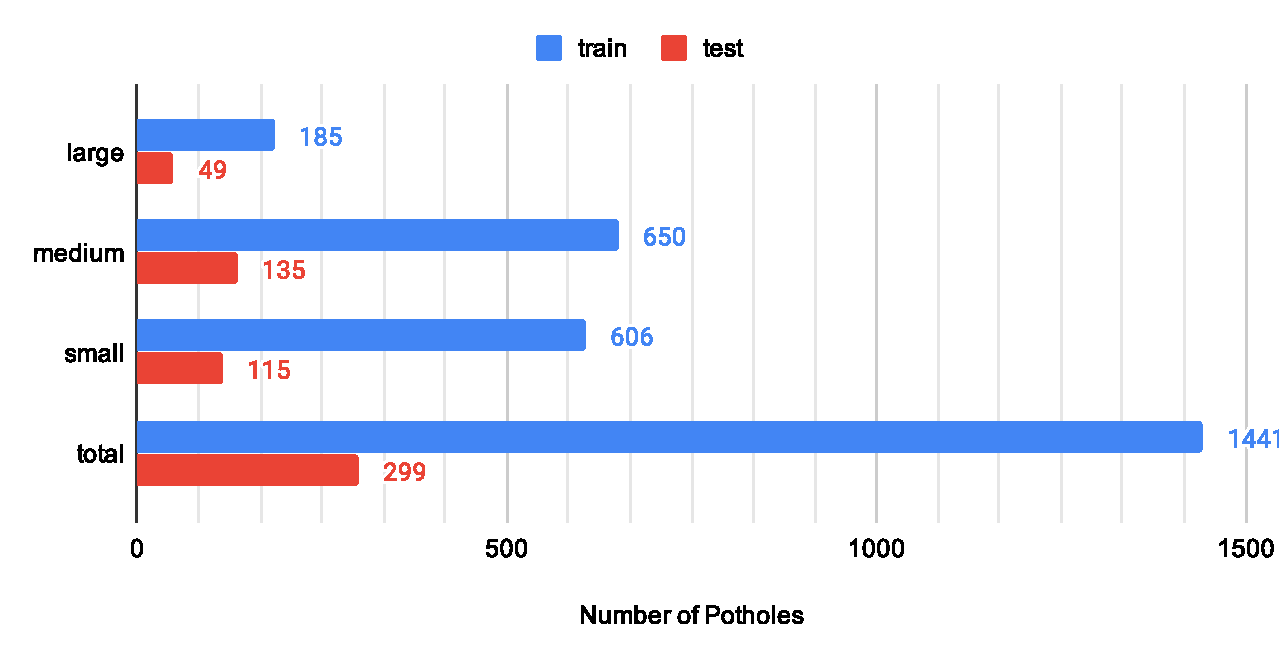
\includegraphics[width=.95\columnwidth]{img/potholes-in-dataset}
  \caption{Distribution of Different Categories of Potholes}
  \label{fig:size_distribution}
\end{figure}

The dataset can be found in \cite{atik2020potholesdataset}.

\subsection{Materials Used}
Basically a transfer learning\cite{pan2009survey} approach was followed in this research to build the target model. Because image data was used, we needed to extract the features of the regions having potholes. To do so, existing pre-trained MobileNet\cite{howard2017mobilenets} model was used as the feature extractor. For the detection task i.e. to predict the bounding boxes around potholes in images, pre-trained Single Shot Multibox Detector (SSD)\cite{liu2016ssd} model was fine-tuned. Both the MobileNet\cite{howard2017mobilenets} and SSD are based on Convolutional Neural Network. Although MobileNet\cite{howard2017mobilenets} has a lower classification performance compared to other larger models\cite{tf_model_zoo}, it is worthwhile for ``real-time'' operation purpose on low-end devices like android mobile-phones and embedded devices.
Architecture of the SSD MobileNet\cite{liu2016ssd, howard2017mobilenets} is shown in Figure \ref{fig:ssd}.
     
\begin{figure}[h]
  \centering
  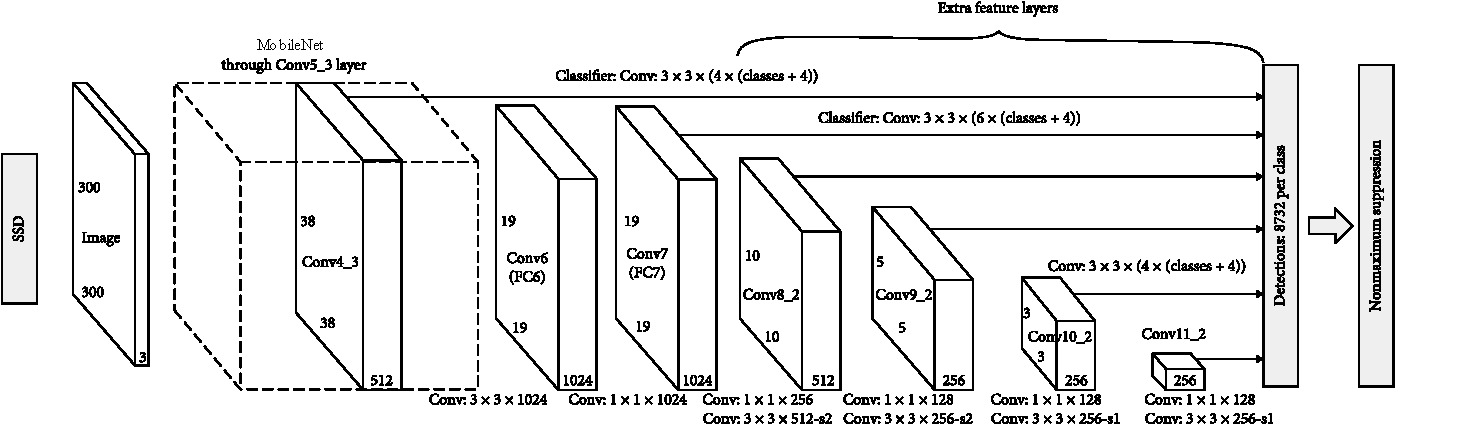
\includegraphics[width=.95\columnwidth]{img/ssd}
  \caption{Architecture of the SSD MobileNet Model}
  \label{fig:ssd}
\end{figure}
     
With the help of Tensorflow\cite{dillon2017tensorflow} Object Detection API, the model was trained using the prepared dataset with some fine-tuned configurations. Figure \ref{fig:workflow} illustrates the interaction of different components during training. The whole model was trained and evaluated on the Google Colaboratory\cite{bisong2019google}.
     
\begin{figure}[h]
  \centering
  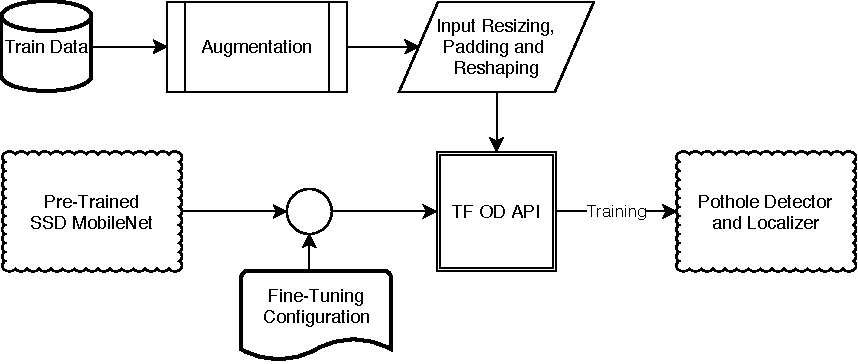
\includegraphics[width=.98\columnwidth]{img/workflow}
  \caption{Interaction of Different Training Components}
  \label{fig:workflow}
\end{figure}
     
\subsection{Training the Model}
\subsubsection{Data Augmentation}
The training images were augmented in different ways. The following augmentations were applied on the training images on-line i.e. during training phase---
\begin{itemize}
  \item Horizontal Flip
  \item Random Crop
  \item Resize Keeping the Aspect Ratio.
  \item Zero Padding
\end{itemize}
      
\subsubsection{Input Resizing}
The shape of the input layer of our model is 300x300x3, that is, it takes RGB images of 300px width and 300px height. But the dataset contains different sizes of images, even a large portion of the images is not square-shaped. Therefore, it was obvious to make the input shape similar as the model's input shape. To address this, we have resized the input such a way that the longer-side was resized to 300px and the shorter size was resized keeping the aspect ratio intact. The remaining space of the shorter side was filled with zeros.
      
\subsubsection{Preparing a Pre-Trained Model}
We have followed transfer learning approach\cite{pan2009survey} in this research experiment. So, we required a pre-trained model ready to be used as a base model. There are many pre-trained models trained on different datasets with different metrics. These pre-trained models can be found in Tensorflow\cite{dillon2017tensorflow} Model Zoo\cite{tf_model_zoo}.
        
We have used the SSD\cite{liu2016ssd} MobileNet\cite{howard2017mobilenets} V2 pre-trained model which was trained on Microsoft COCO dataset\cite{lin2014microsoft}.
        
Every pre-trained model in the Tensorflow Model Zoo\cite{tf_model_zoo} contains a ``pipeline.config'' file which is used as a configuration file during training and evaluation. We have removed/changed/added several configuration options in that file. Our changes are shown in table \ref{tab:fine_tuned_conf}.
        
Some of the options the configuration file consists---
\begin{itemize}
  \item Number of classes or labels
  \item Activation Functions
  \item Prepossessing and Data Augmentation Options
  \item Learning Rate and Batch Size
  \item Evaluation Methods
\end{itemize}
            
\begin{table}[h]
  \centering
  \caption{Fine-Tuned Configurations}
  \label{tab:fine_tuned_conf}    \renewcommand{\arraystretch}{1.3}
  \begin{tabular}{l||l}
    \bfseries{Configuration Option} & \bfseries{Changed Value}     \\\hline\hline
    input\_shape                    & (300, 300, 3)                \\\hline
    num\_classes                    & 1                            \\\hline
    batch\_size                     & 24                           \\\hline
    image\_resizer                  & keep\_aspect\_ratio\_resizer \\\hline
    min\_dimension                  & 300                          \\\hline
    max\_dimension                  & 300                          \\\hline
    pad\_to\_max\_dimension         & true                         \\\hline
    initial\_learning\_rate         & 0.005                        \\\hline
    decay\_steps                    & 6000                         \\\hline
    decay\_factor                   & 0.85                         \\\hline
    quantization\_delay             & 30000                        \\\hline
  \end{tabular}
\end{table}
      
\subsubsection{Prepare Tensorflow Models Repository}
For the purpose of training as well as validation of our model we reused the existing libraries, packages and codes from the Tensorflow ``models'' repository\cite{tf_models_repo}. The repository contains almost everything we need for training and evaluation using Tensorflow API. The mentioned repository can be found in Github\cite{tf_models_repo}.
    
\subsubsection{Run Training Process}
Tensorflow ``models'' repository provides necessary python code for the whole training process. It also saves the checkpoints of the model in training at a regular interval of time. It starts training from the saved checkpoints if the process is interrupted\cite{tf_models_repo}. It saves the scalar and graphical values i.e. the results of training and evaluation in ``tfevent'' files which can be monitored in Tensorboard\cite{manetensorboard}.

\begin{figure}
  \centering
  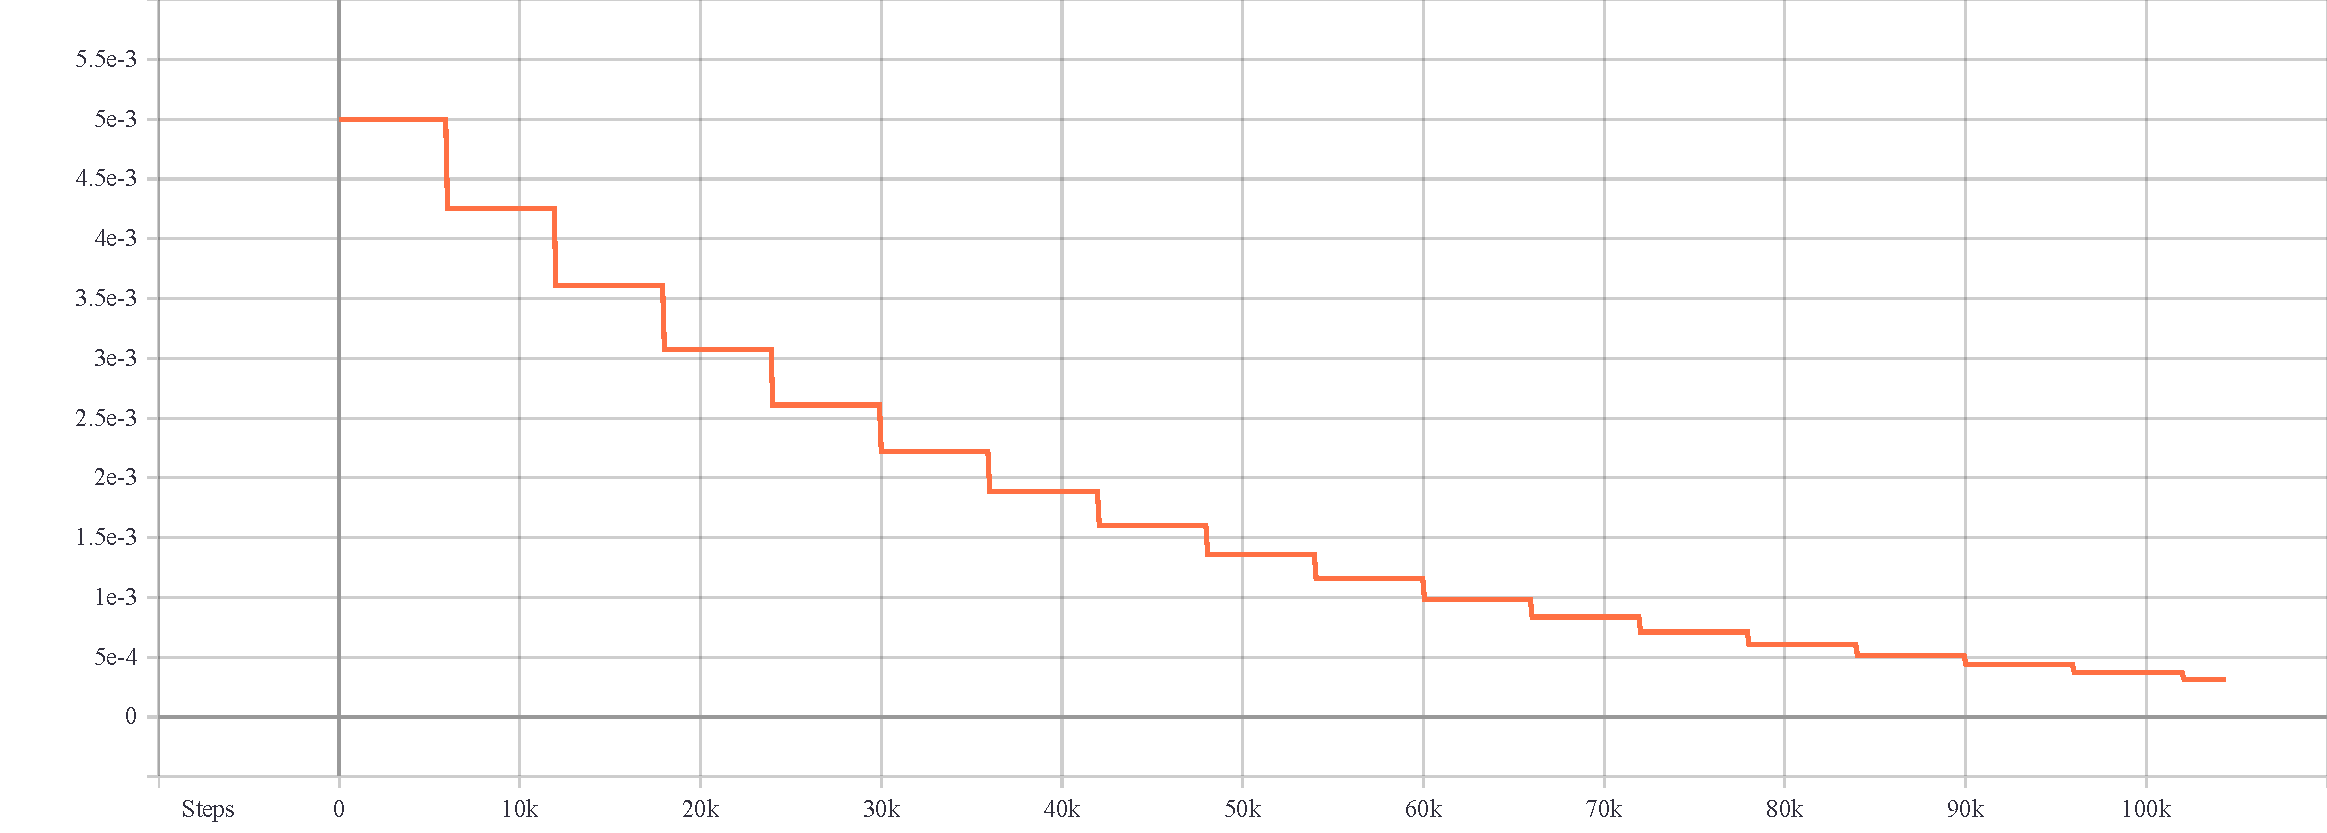
\includegraphics[width=.98\columnwidth]{img/learning_rate}
  \caption{Training Steps vs Decay of Learning Rate}
  \label{fig:learning_rate}
\end{figure}        
        
\subsubsection{Run Evaluation Process}
After the training process ends, we can run the evaluation on the validation dataset. Tensorflow ``models'' repository provides the tools for the evaluation process too. The evaluation is triggered by the training tool automatically whenever it saves a checkpoint of the model\cite{tf_models_repo}. This helps to monitor the performance of the model at different levels of training steps and epochs.
 
\subsection{Evaluation Methods}
\subsubsection{Intersection Over Union (IoU)}
To evaluate the performance of the model, precision and recall values were used. To take a detected bounding-box as true positive, different Intersection over Union (IoU) thresholds were considered.
    
\begin{figure}[h]
  \centering
  \includegraphics[height=3cm]{img/IoU}
  \caption{Measuring the Intersection over Union (IoU)}
  \label{fig:iou}
\end{figure}
    
Following IoU thresholds were considered---
\begin{itemize}
  \item IoU@50\%
  \item IoU@75\%
  \item IoU@50\%:5\%:95\%
\end{itemize}
IoU@50\%:5\%:95\% is a dynamic measurement where 10 IoU thresholds are considered, starting from 50\%, upto 95\% with an interval of 5\%, following thresholds are found--- 50\%, 55\%, 60\%, 65\%, 70\%, 75\%, 80\%, 85\%, 90\%, 95\%. Values at these 10 thresholds were then averaged to get the value for IoU@50\%:5\%:95\%.
    
Here, taking the above IoU thresholds into account, \\
$TP$ = Number of True Positive Predictions \\
$FP$ = Number of False Positive Predictions \\
$TN$ = Number of True Negative Predictions \\
$FN$ = Number of False Negative Predictions\\
    
\subsubsection{Precision Calculation}
Precision shows how much the predictions are correct\cite{buckland1994relationship}. That is, percentage of correct predictions among all the positive-predicted values.  
    
\begin{equation}   
  Precision = \frac{TP}{TP+FP}    
\end{equation}
    
Average Precision is the area under precision-recall curve.
\begin{equation}
  AP = \int_{0}^{1}p(r) ~dr
\end{equation}
Here, $r$ represents recall, $p$ represents precision as a function of $r$. Therefore, $p(r)$ means ``precision at recall $r$''.
    
In this research, only a single class is available and it is labeled ``pothole'', therefore, Mean Average Precision (mAP) is same as Average Precision (AP). For multi-class, mAP is the mean of Average Precisions of all individual classes.
\begin{equation}
  mAP = \frac{1}{N} \sum_{i=1}^N AP_i
\end{equation}
Here, $mAP$ is Mean Average Precision, $N$ is the number of class-labels, $AP_i$ is the Average Precision for $i^{th}$ class.

We considered and calculated mean average precision for different  sizes of potholes as well as for different IoU thresholds---
\begin{itemize}
  \item mAP@50\% IoU
  \item mAP@75\% IoU
  \item mAP@50\%:5\%:95\% IoU for small sizes.
  \item mAP@50\%:5\%:95\% IoU for medium sizes.
  \item mAP@50\%:5\%:95\% IoU for large sizes.
  \item mAP@50\%:5\%:95\% IoU for all sizes.
\end{itemize}  
  
\subsubsection{Recall Calculation}
Recall means True Positive Rate and also known as sensitivity, a well-known parameter (measurement) for model evaluation in the context of classification\cite{wiki:precision_recall}.
            
We considered and calculated average recall for different  sizes of potholes as well as for different maximum detection levels---
\begin{itemize}
  \item AR@1 detection
  \item AR@10 detections
  \item AR@100 detection for small sizes
  \item AR@100 detection for medium sizes
  \item AR@100 detection for large sizes
  \item AR@100 detections for all sizes
\end{itemize}
Average Recall is same as Recall in this research because, there is a single class-label in the dataset, namely, ``pothole''.
All of these recall values were calculated for 50\%:5\%:95\% IoU threshold, i.e. using MS COCO metrics\cite{lin2014microsoft}.
    
\begin{equation}   
  Recall = \frac{TP}{TP+FN}
\end{equation}
    
Average Recall is the mean of the recall values of all individual classes.
\begin{equation}
  AR = \frac{1}{N} \sum_{i=1}^N r_i
\end{equation}
Here, $AR$ is Average Recall, $N$ is the number of class-labels, $r_i$ is the Recall for $i^{th}$ class.
        
%%%%%%%%%%%%%%%%%%% Results %%%%%%%%%%%%%%%%%%%
\section{Results and Discussion}
The training process was run for more than 100,000 steps with a batch size of 24. Then evaluation process was run with the help of the Tensorflow ``models'' repository. The evaluation process used the performance metrics following the Microsoft Common Objects in Context (COCO)\cite{lin2014microsoft}.
  
Precision values found on the test dataset after more than 100,000 steps of training are shown here in tabular form as well as using bar-charts.
  
\subsection{Average Precision for Different IoU Thresholds}
In TABLE ~\ref{tab:precision_iou}, the model's performance is shown as Average Precision considering different minimum IoU thresholds as the threshold for True Positive detection.
\begin{table}[h]
  \centering
  \caption{Precision at Different IoU Thresholds}
  \label{tab:precision_iou}
  \renewcommand{\arraystretch}{1.3}
  \begin{tabular}{c||c}
    \bfseries{IoU Threshold} & \bfseries{Precision on Validation Data} \\\hline\hline
    50\%                     & 0.65                                    \\\hline
    75\%                     & 0.36                                    \\\hline
    50\%:5\%:90\%            & 0.37                                    \\\hline
  \end{tabular}
\end{table}
  
\subsection{Average Precision for Different Pothole-Sizes}
In TABLE ~\ref{tab:precision_sizes}, the model's performance is shown as Average Precision considering different categories of pothole sizes in the test-dataset.
    
\begin{table}[h]
  \centering
  \caption{Precision for Different Pothole-Sizes}
  \label{tab:precision_sizes}
  \renewcommand{\arraystretch}{1.3}
  \begin{tabular}{l||c}
    \bfseries{Area Sizes} & \bfseries{Precision on Validation Data} \\\hline\hline
    Small                 & 0.07                                    \\\hline
    Medium                & 0.26                                    \\\hline
    Large                 & 0.58                                    \\\hline
  \end{tabular}
\end{table}
  
Figure \ref{fig:mAP} summarizes the Mean Average Precision values considering different IoU thresholds and different pothole size-categories.
  
\begin{figure}[h]
  \centering
  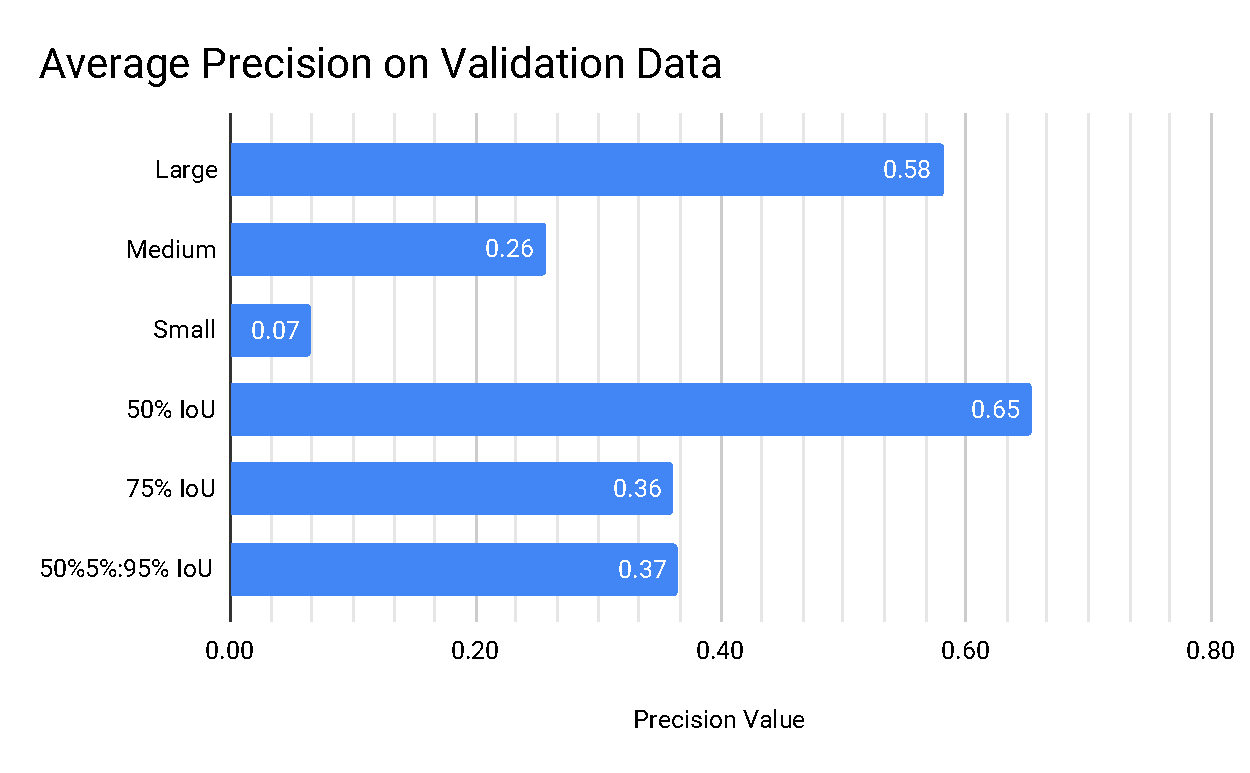
\includegraphics[width=.95\columnwidth]{img/Average-Precision-on-Validation-Data}
  \caption{Average Precision on Validation Data}
  \label{fig:mAP}
\end{figure}
  
\subsection{Average Recall at Different Detection Limits}
We have taken the recall values at different limits of maximum detections. More specifically, we have taken the following limits for the calculation of recall values---
\begin{itemize}
  \item {Average Recall at maximum of 1 detection (AR@1)}
  \item {Average Recall at maximum of 10 detections (AR@10)}
  \item {Average Recall at maximum of 100 detection (AR@100)}
\end{itemize}
   
In TABLE ~\ref{tab:recall_limits}, Average Recall values are shown for different detection limits.
\begin{table}[h]
  \centering
  \caption{Recall for Different Detection-Limits}
  \label{tab:recall_limits}
  \renewcommand{\arraystretch}{1.3}
  \begin{tabular}{c||c} 
    \bfseries{Maximum Detections} & \bfseries{Recall on Validation Data} \\\hline\hline
    1                             & 0.27                                 \\\hline
    10                            & 0.44                                 \\\hline
    100                           & 0.49                                 \\\hline
  \end{tabular}
\end{table}
    
\subsection{Average Recall for Different Pothole-Sizes}
In TABLE ~\ref{tab:recall_sizes}, Average Recall values are shown for different categories of pothole sizes. Here, all the values are calculated at the threshold of IoU@50\%:5\%:95\%.
    
\begin{table}[h]
  \centering
  \caption{Recalls for Different Pothole-Sizes}
  \label{tab:recall_sizes}
  \renewcommand{\arraystretch}{1.3}
  \begin{tabular}{l||c}
    \bfseries{Area Sizes} & \bfseries{Recall on Validation Data} \\\hline\hline
    Small                 & 0.18                                 \\\hline
    Medium                & 0.44                                 \\\hline
    Large                 & 0.67                                 \\\hline
  \end{tabular}
\end{table} 
    
Figure \ref{fig:AR}, summarizes all the Average Recall values as measures of performance for the model. Here, all detections were calculated with IoU@50\%:5\%:95\% threshold.
    
\begin{figure}[h]
  \centering
  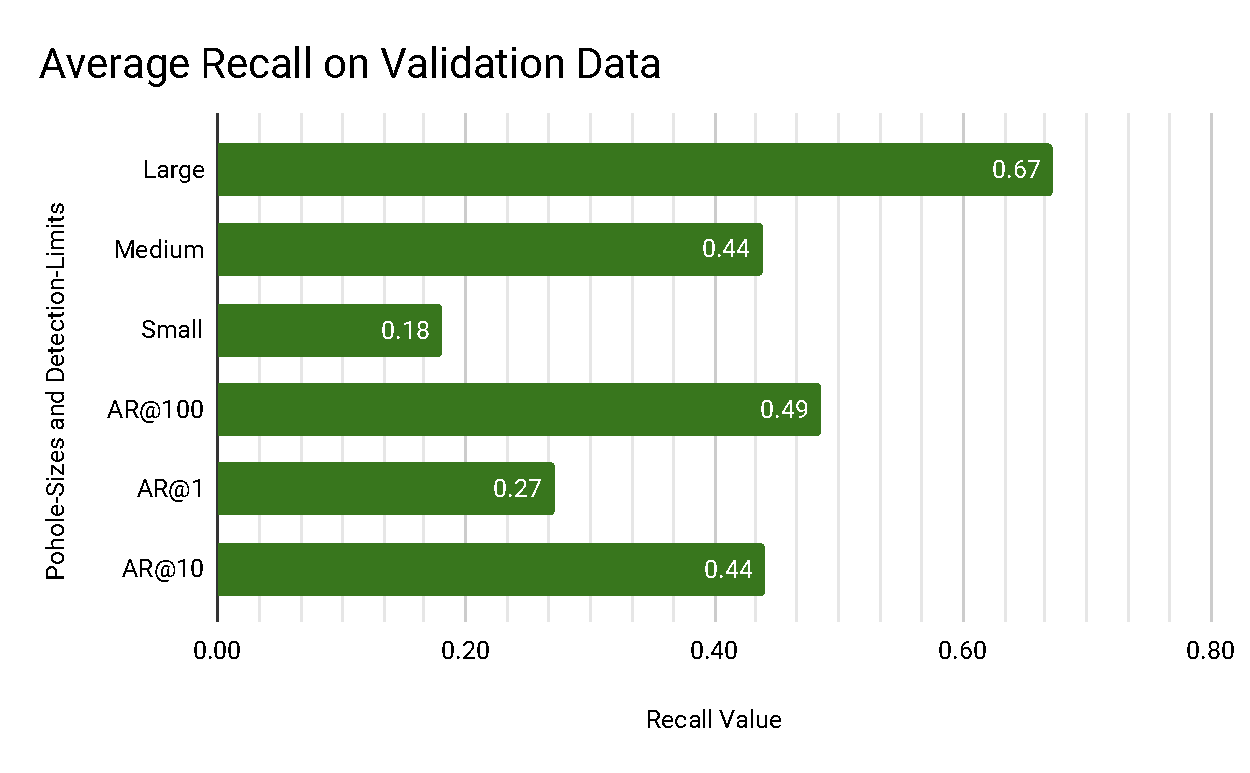
\includegraphics[width=.95\columnwidth]{img/Average-Recall-on-Validation-Data}
  \caption{Average Recall on Validation Data}
  \label{fig:AR}
\end{figure}
      
From figures \ref{fig:mAP} and \ref{fig:AR}, it is clear that the model performs better for larger potholes. Although the precision values are not very high, it is worth accepting because of such a light-weight model like MobileNet SSD which is built targeting the low-end mobile devices\cite{howard2017mobilenets}.
  
%%%%%%%%%%%%%%%%%%% Conclusions %%%%%%%%%%%%%%%%%%%
\section{Conclusion and Future Works}
Considering the severity of potholes, a system was developed to automatically detect them in real-time and generate warning signals to help for avoidance. A deep convolutional neural network model named ``MobileNet'' was used as feature extractor applying a transfer learning mechanism. ``Single Shot Multibox Detector'' model was fine-tuned for pothole detection and localization. An android application was developed using the model which can detect, localize and track the potholes in real-time analyzing the video frames. The app generates warning signal as long as it detects pothole in the video frames coming from its camera. So, the system can be used by visually impaired people to avoid potholes while navigating. It can also be used in automated vehicle driving.
  
In future, more research would be accomplished to make the system more accurate, more robust, more intelligent.
  
Research for estimating the distance of the detected potholes would be done in near future. Measuring the severity of the potholes would also be included in future works. Making the model aware of different sizes of potholes may be included as future tasks. Also measurement of dimension like area, depth etc. of the detected pothole would be done in future research.
\\
\vspace{1cm}% To make last page columns equal.
%%%%%%%%%%%%%%%%%%% References %%%%%%%%%%%%%%%%%%%
\IEEEtriggeratref{13}% To make last page columns equal, break at 13th reference.
\bibliographystyle{IEEEtran}
\bibliography{IEEEabrv,references}

\end{document}
